\documentclass[compress,mathserif]{beamer}
\usetheme{sthlm}

%-=-=-=-=-=-=-=-=-=-=-=-=-=-=-=-=-=-=-=-=-=-=-=-=
%        LOADING BEAMER PACKAGES
%-=-=-=-=-=-=-=-=-=-=-=-=-=-=-=-=-=-=-=-=-=-=-=-=

\usepackage{
booktabs,
datetime,
dtk-logos,
graphicx,
multicol,
pgfplots,
ragged2e,
tabularx,
tikz,
wasysym,
multirow,
float,
caption,
subcaption,
amsmath,
mathptmx
}

\usepackage[scaled=0.9]{helvet}
\usepackage{courier}

\usefonttheme[onlymath]{serif}

\definecolor{mygreen}{RGB}{113, 166, 70}
\definecolor{myblue}{RGB}{68, 140, 185}
\definecolor{myred}{RGB}{217, 98, 55}
\definecolor{mypurple}{RGB}{83, 65, 126}
\definecolor{solviaveis}{RGB}{188, 207, 241}

\pgfplotsset{compat=1.8}

\usepackage[utf8]{inputenc}
\usepackage[portuguese]{babel}
\usepackage[T1]{fontenc}
\usepackage{newpxtext,newpxmath}
\usepackage{listings}

\lstset{ %
language=[LaTeX]TeX,
basicstyle=\normalsize\ttfamily,
keywordstyle=,
numbers=left,
numberstyle=\tiny\ttfamily,
stepnumber=1,
showspaces=false,
showstringspaces=false,
showtabs=false,
breaklines=true,
frame=tb,
framerule=0.5pt,
tabsize=4,
framexleftmargin=0.5em,
framexrightmargin=0.5em,
xleftmargin=0.5em,
xrightmargin=0.5em
}



%-=-=-=-=-=-=-=-=-=-=-=-=-=-=-=-=-=-=-=-=-=-=-=-=
%        LOADING TIKZ LIBRARIES
%-=-=-=-=-=-=-=-=-=-=-=-=-=-=-=-=-=-=-=-=-=-=-=-=

\usetikzlibrary{
backgrounds,
mindmap
}

%-=-=-=-=-=-=-=-=-=-=-=-=-=-=-=-=-=-=-=-=-=-=-=-=
%        BEAMER OPTIONS
%-=-=-=-=-=-=-=-=-=-=-=-=-=-=-=-=-=-=-=-=-=-=-=-=

\setbeameroption{show notes}

%-=-=-=-=-=-=-=-=-=-=-=-=-=-=-=-=-=-=-=-=-=-=-=-=
%        BEAMER COMMANDS
%-=-=-=-=-=-=-=-=-=-=-=-=-=-=-=-=-=-=-=-=-=-=-=-=


%-=-=-=-=-=-=-=-=-=-=-=-=-=-=-=-=-=-=-=-=-=-=-=-=
%
%	PRESENTATION INFORMATION
%
%-=-=-=-=-=-=-=-=-=-=-=-=-=-=-=-=-=-=-=-=-=-=-=-=

\title{Modelagem de problemas usando Programação Linear}
\subtitle{DCE692 - Pesquisa Operacional}
%\date{\small{\jobname}}
\author{\texttt{Iago Carvalho}}
\institute{\texttt{Departamento de Ciência da Computação}}

\hypersetup{
pdfauthor = {Iago A. Carvalho},      
pdfsubject = {Pesquisa Operacional},
pdfkeywords = {},  
pdfmoddate= {D:\pdfdate},          
pdfcreator = {WriteLaTeX}
}

\begin{document}

\begin{frame}
\titlepage

\end{frame}

%% --------------------------------------------------------

\begin{frame}{Modelagem de problemas}

É a \textit{arte} de descrever um problema de otimização como um conjunto de equações
\begin{itemize}
    \item Função objetivo
    \item Variáveis
    \item Restrições
\end{itemize}

\vspace{0.5cm}

Como estamos trabalhando com Programação Linear, então temos que garantir que
\begin{itemize}
    \item Variáveis pertencem ao domínio dos reais $(\mathbb{R}$)
    \item Função objetivo e restrições são lineares
\end{itemize}
\end{frame}

%% --------------------------------------------------------

\begin{frame}{Modelagem de problemas}

Como toda arte, a modelagem de problemas é muito difícil de ser ensinada
\begin{itemize}
    \item A maneira mais simples é através da prática, de exemplos e de observação
\end{itemize}

\vspace{0.5cm}

Deste modo, vamos tentar aprender modelagem através de exemplos!

\begin{columns}[T]
    \begin{column}{.49\textwidth}
        \begin{itemize}
            \item Problema da dieta
            \item Problema de corte
        \end{itemize}
    \end{column}
    \begin{column}{.49\textwidth}
        \begin{itemize}
            \item Problema do transporte
            \item Escala de funcionários
        \end{itemize}
    \end{column}
\end{columns}
\end{frame}

%% --------------------------------------------------------

\begin{frame}{Problema da dieta}

Este foi um dos primeiros problemas de Otimização Linear estudados \href{https://neos-guide.org/content/diet-problem}{\beamergotobutton{Link}}

\begin{itemize}
    \item Segunda guerra mundial
    \item Criar um conjunto de refeições baratas
    \item Requisitos nutricionais eram atendidos
\end{itemize}

\centering 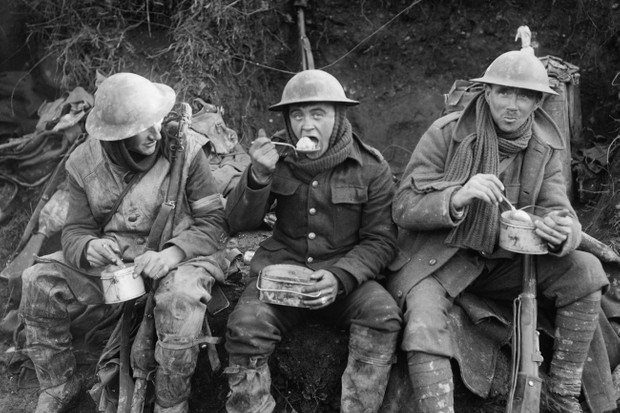
\includegraphics[width=\textwidth]{images/soldier_eating.jpg}

\end{frame}

%% --------------------------------------------------------

\begin{frame}{Problema da dieta}

\begin{table}[]
\def\arraystretch{1.8}
\centering
\resizebox{\textwidth}{!}{%
\begin{tabular}{@{}ccccccc@{}}
\toprule
\textbf{Alimento} & \textbf{Porção} & \textbf{Calorias (kcal)} & \textbf{Proteínas (g)} & \textbf{Calcio (mg)} & \textbf{Preço (\$)} & \textbf{Limite} \\ \midrule
Nozes  & 28 g        & 110 & 4  & 2   & 30  & 4 \\
Frango & 100 g       & 205 & 32 & 12  & 240 & 3 \\
Ovos   & 2 (grandes) & 160 & 13 & 54  & 130 & 2 \\
Leite  & 237 ml      & 160 & 8  & 285 & 90  & 8 \\
Bolo   & 170 g       & 420 & 4  & 22  & 200 & 2 \\
Feijão & 260 g       & 260 & 14 & 80  & 60  & 2 \\ \bottomrule
\end{tabular}%
}
\end{table}

\end{frame}

%% --------------------------------------------------------

\begin{frame}{Problema da dieta}

Conjuntos: \\
\vspace{0.2cm}
$\begin{matrix}
F & \textnormal{Conjunto de alimentos} \\
N & \textnormal{Conjunto de nutrientes}
\end{matrix} 
$

\vspace{1cm}

Parâmetros: \\
\vspace{0.2cm}
$\begin{matrix}
a_{ij} & \textnormal{Quantidade do nutriente } j \textnormal{ no alimento } i, & \forall i \in F, j \in N\\
c_i & \textnormal{Custo de uma porção do alimento } i, & \forall i \in F \\
m_j & \textnormal{Requisito mínimo do nutriente } j, & \forall j \in N
\end{matrix}
$

\vspace{1cm}

Variáveis: \\
\vspace{0.2cm}
$\begin{matrix}
x_i \geq 0 & \textnormal{Quantidade servida do alimento } i, & \forall i \in F
\end{matrix}
$

\end{frame}

%% --------------------------------------------------------

\begin{frame}{Problema da dieta}

$$\begin{matrix}
        \min & \sum_{i \in F}~x_i\,c_i\\  \\
             & \sum_{i \in F}~x_i\,a_{ij} & \geq m_j, & \forall j \in N \\ \\
             & x_i & \geq 0 & \forall i \in F
        \end{matrix}    
$$

\end{frame}

%% --------------------------------------------------------

\begin{frame}{Problema do corte de produtos}

Problema do corte de produtos teve suas origens na indústria de papéis \href{https://neos-guide.org/content/cutting-stock-problem}{\beamergotobutton{Link}}

\begin{itemize}
    \item Rolos de papel muito grandes, de dimensões fixas
    \item Deve-se cortar estes rolos em itens menores
    \begin{itemize}
        \item Diferentes tamanhos
        \item 1D
    \end{itemize}
    \item O objetivo é cortar todos os itens pedidos
    \begin{itemize}
        \item Minimizar a quantidade de perda de papel
    \end{itemize}
\end{itemize}
\end{frame}

%% --------------------------------------------------------

\begin{frame}{Problema do corte de produtos}

\vspace{1cm}
\centering 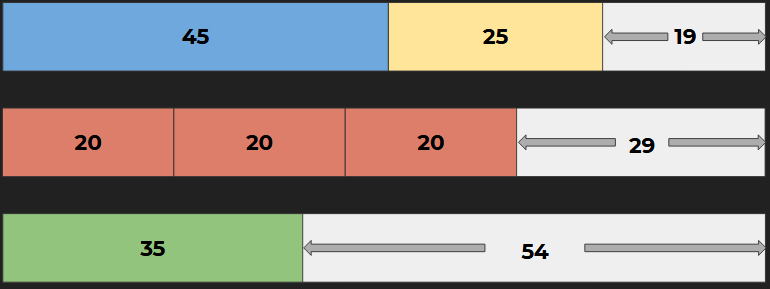
\includegraphics[width=\textwidth]{images/cutting_1d.png}

\end{frame}

%% --------------------------------------------------------

\begin{frame}{Problema do corte de produtos}

Conjuntos: \\
\vspace{0.2cm}
$\begin{matrix}
I & \textnormal{Conjunto de tamanho dos pedidos} \\
J & \textnormal{Conjunto de padrões de corte}
\end{matrix} 
$

\vspace{1cm}

Parâmetros: \\
\vspace{0.2cm}
$\begin{matrix}
a_{ij} & \textnormal{Número de itens de tamanho } i \textnormal{ no padrão } j, & \forall i \in I, j \in J\\
b_i & \textnormal{Demanda por itens de tamanho } i, & \forall i \in I
\end{matrix}
$

\vspace{1cm}

Variáveis: \\
\vspace{0.2cm}
$\begin{matrix}
x_j \in \mathbb{I}_{\geq 0} & \textnormal{Número de padrões de corte } j \textnormal{ utilizados}, & \forall j \in J
\end{matrix}
$

\end{frame}

%% --------------------------------------------------------

\begin{frame}{Problema do corte de produtos}

$$\begin{matrix}
        \min & \sum_{j \in J}~x_j\\  \\
             & \sum_{j \in J}~x_j\,a_{ij} & \geq b_i, & \forall i \in I \\ \\
             & x_j & \geq 0 & \forall j \in J
        \end{matrix}    
$$

\end{frame}

%% --------------------------------------------------------

\begin{frame}{Problema do transporte}

Uma empresa produz um produto em diversas fábricas \href{http://www.producao.ufrgs.br/arquivos/disciplinas/382_winston_cap_7_transportation.pdf}{\beamergotobutton{Link}}
\begin{itemize}
    \item Diferentes clientes demandam os produtos
\end{itemize}
 
\vspace{0.5cm}
 
O objetivo é entregar os produtos a todos os clientes
\begin{itemize}
    \item Atender a todas as demandas
    \item Minimizar os custos de entrega
    \begin{itemize}
        \item Dependentes da distância entre a fábrica e o cliente
    \end{itemize}
\end{itemize}
\end{frame}

%% --------------------------------------------------------

\begin{frame}{Problema do transporte}

\vspace{1cm}
\centering 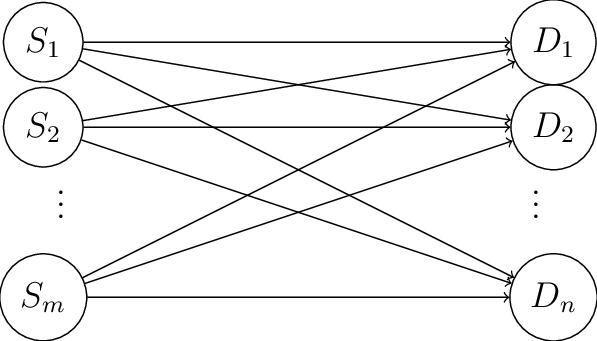
\includegraphics[width=0.9\textwidth]{images/transporte.png}

\end{frame}

%% --------------------------------------------------------

\begin{frame}{Problema do transporte}

Conjuntos: \\
\vspace{0.2cm}
$\begin{matrix}
F & \textnormal{Conjunto de fábricas} \\
C & \textnormal{Conjunto de clientes}
\end{matrix} 
$

\vspace{1cm}

Parâmetros: \\
\vspace{0.2cm}
$\begin{matrix}
a_{i} & \textnormal{Produção disponível na fábrica } i, & \forall i \in F\\
b_j & \textnormal{Demanda do cliente } j, & \forall j \in C \\
c_{ij} & \textnormal{Custo de entrega entre a fábrica } i \textnormal{ e o cliente } j, & \forall i \in F, j \in C
\end{matrix}
$

\vspace{1cm}

Variáveis: \\
\vspace{0.2cm}
$\begin{matrix}
x_{ij} \geq 0 & \textnormal{Volume de entregas da fábrica } i \textnormal{ para o cliente } j, & \forall i \in F, j \in C
\end{matrix}
$

\end{frame}

%% --------------------------------------------------------

\begin{frame}{Problema do transporte}

$$\begin{matrix}
        \min & \sum_{i \in F} \sum_{j \in C}~c_{ij}\,x_{ij}\\  \\
             & \sum_{j \in C}~x_{ij} & \leq a_i, & \forall i \in F \\ \\
             & \sum_{i \in F}~x_{ij} & \geq b_j & \forall j \in C \\ \\
             & x_{ij} & \geq 0 & \forall i \in F, j \in C
        \end{matrix}    
$$

\end{frame}



%% --------------------------------------------------------

\begin{frame}{Escala de funcionários}

Uma companhia aérea deseja abrir novas rotas
\begin{itemize}
    \item Origem ou destino em seu aeroporto base
\end{itemize}
 
\vspace{0.5cm}
 
Para isto, é necessário contratar mais funcionários
\begin{itemize}
    \item Alocar funcionários nas novas rotas
    \begin{itemize}
        \item Dependente do horário das rotas
    \end{itemize}
\end{itemize}

\vspace{0.5cm}

Vamos fazer um pouco diferente desta vez... 
\begin{itemize}
    \item Vamos mostrar um caso numérico!
\end{itemize}

\end{frame}

%% --------------------------------------------------------

\begin{frame}{Escala de funcionários}

\begin{table}[]
\centering
\resizebox{\textwidth}{!}{%
\begin{tabular}{@{}ccccccc@{}}
\toprule
         & \multicolumn{5}{c}{Turno}        &                      \\ \cmidrule(l){2-6} 
Horários & 1   & 2   & 3   & 4   & 5   & Funcionários necessários \\ \midrule
6-8      & x   &     &     &     &     & 48                       \\
8-10     & x   & x   &     &     &     & 79                       \\
10-12    & x   & x   &     &     &     & 65                       \\
12-14    & x   & x   & x   &     &     & 87                       \\
14-16    &     & x   & x   &     &     & 64                       \\
16-18    &     &     & x   & x   &     & 73                       \\
18-20    &     &     & x   & x   &     & 82                       \\
20-22    &     &     &     & x   &     & 43                       \\
22-24    &     &     &     & x   & x   & 52                       \\
24-06    &     &     &     &     & x   & 15                       \\ \midrule
Custo    & 170 & 160 & 175 & 180 & 195 &                          \\ \bottomrule
\end{tabular}%
}
\end{table}

\end{frame}

%% --------------------------------------------------------

\begin{frame}{Escala de funcionários}

Considere a variável
$$\begin{matrix}
x_{i} \geq 0 & \textnormal{Número de funcionários alocados no turno } i , & i \in \{1, 2, 3, 4, 5\}
\end{matrix}$$

\end{frame}

%% --------------------------------------------------------

\begin{frame}{Problema do corte de produtos}

$$\begin{matrix}
        \min & 170\,x_1 + 160\,x_2 + 175\,x_3 + 180\,x_4 + 195\,x_5\\  
             & x_1             & \geq 48 & (6-8) \\ 
             & x_1 + x_2       & \geq 79 & (8-10) \\ 
             & x_1 + x_2       & \geq 65 & (10-12) \\ 
             & x_1 + x_2 + x_3 & \geq 87 & (12-14) \\ 
             & x_2 + x_3       & \geq 64 & (14-16) \\ 
             & x_3 + x_4       & \geq 73 & (16-18) \\ 
             & x_3 + x_4       & \geq 82 & (18-20) \\ 
             & x_4             & \geq 43 & (20-22) \\ 
             & x_4 + x_5       & \geq 52 & (22-24) \\ 
             & x_5             & \geq 15 & (24-6) \\ 
             & x_i & \geq 0 & i \in \{1, 2, 3, 4, 5\}
        \end{matrix}    
$$

\end{frame}

%% --------------------------------------------------------

\begin{frame}{Outros problemas}


Problema de atribuição de tarefas
\begin{itemize}
    \item Resolvido como um problema de transporte
\end{itemize}

\vspace{1cm}

Problema do máximo fluxo em redes
\begin{itemize}
    \item Um caso mais específico (e difícil) do problema de transporte
\end{itemize}


\end{frame}

\end{document}